% ============================================================================
% CAPÍTULO 5 — RESULTADOS E DISCUSSÃO
% ============================================================================

\chapter{Resultados e Discussão}
\label{cap:resultados}

Este capítulo apresenta os resultados obtidos com a aplicação do pipeline desenvolvido, organizados segundo as etapas do fluxo de trabalho. Diferentemente da versão anterior deste trabalho, que apresentava resultados esperados de natureza projetiva, os dados aqui descritos são produtos reais de execuções completas do pipeline, validando sua funcionalidade e robustez.

\section{Execuções Realizadas}

O pipeline foi executado para duas espécies, com objetivos complementares. A Tabela~\ref{tab:execucoes} sintetiza os parâmetros e configurações utilizados em cada execução.

\begin{longtable}{@{}p{3.8cm}p{5.2cm}p{5.2cm}@{}}
\caption{Parâmetros de execução do pipeline para as duas espécies analisadas.}
\label{tab:execucoes} \\
\toprule
\textbf{Parâmetro} & \textbf{\textit{Anodorhynchus leari}} & \textbf{\textit{Diploprion bifasciatus}} \\
\midrule
\endfirsthead
\caption[]{Parâmetros de execução do pipeline (continuação).} \\
\toprule
\textbf{Parâmetro} & \textbf{\textit{A.~leari}} & \textbf{\textit{D.~bifasciatus}} \\
\midrule
\endhead
\bottomrule
\endfoot
Objetivo & Objeto principal do TCC & Validação do pipeline \\
\addlinespace
Dataset SRA & SRR28399504 & SRR36182901 \\
\addlinespace
Plataforma & Illumina HiSeq X Ten & NovaSeq X Plus \\
\addlinespace
Leituras & 118,5M $\times$ 150 bp & 12,0M $\times$ 151 bp \\
\addlinespace
Semente & cox1 \textit{A.~hyacinthinus} (NC\_082165.1, 1.548 bp) & cox1 \textit{D.~bifasciatus} (PZ143763.1, 1.560 bp) \\
\addlinespace
\texttt{genome\_range} & 15.500--18.500 bp & 15.000--18.500 bp \\
\addlinespace
K-mers & 39, 33 & 33 \\
\addlinespace
Código genético & 2 (vertebrado) & 2 (vertebrado) \\
\addlinespace
MITOS2 & Sim (RefSeq89m) & Não (perfil de teste sem banco) \\
\addlinespace
Perfil & \texttt{-profile a\_leari} & \texttt{-profile test} \\
\end{longtable}

\section{Aquisição e Preparo dos Dados}

Para a arara-azul-de-lear, o download via \texttt{prefetch} obteve o arquivo \texttt{.sra} de 11~GB, que foi convertido pelo \texttt{fasterq-dump} em dois arquivos FASTQ de aproximadamente 43,5~GB cada (R1 e R2). Após a truncagem para 20 milhões de leituras, os arquivos foram reduzidos para $\sim$7,4~GB cada, representando uma economia de 83\% em volume de dados processados sem qualquer prejuízo à montagem, dada a redundância intrínseca dos dados de genoma total.

\begin{figure}[H]
    \centering
    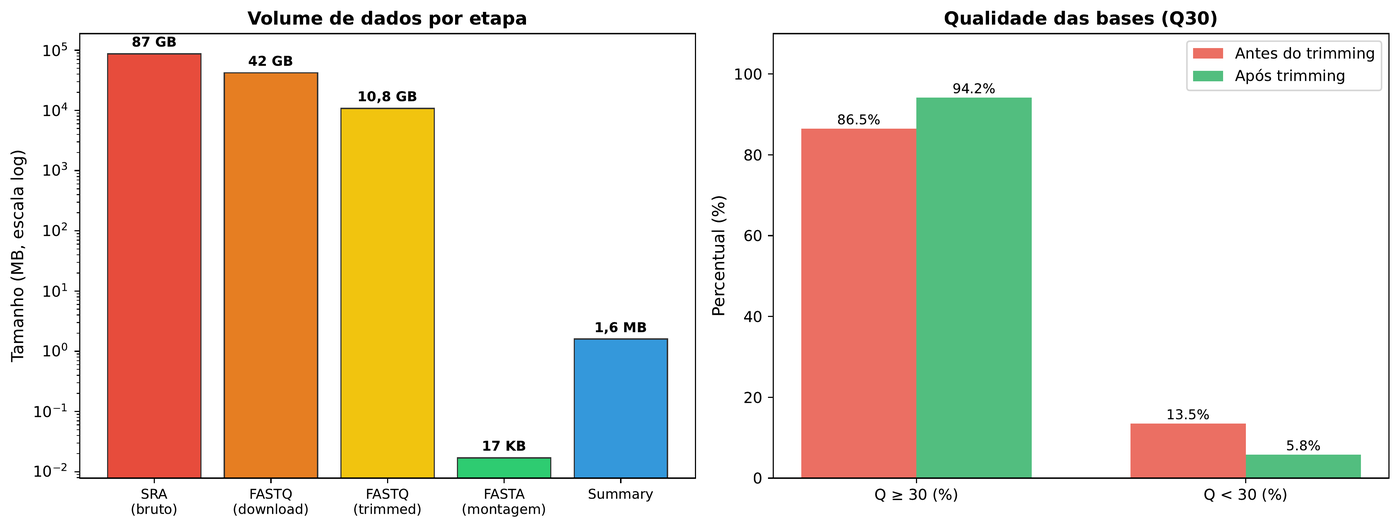
\includegraphics[width=0.85\textwidth]{imagens/reducao_volume_composicao.png}
    \caption{Redução de volume em cada etapa do pipeline para a arara-azul-de-lear: tamanho dos arquivos por etapa (esquerda) e composição de bases após trimming (direita).}
    \label{fig:reducao_volume}
\end{figure}

Para \textit{D.~bifasciatus}, o dataset compacto (12M reads, $\sim$1,2~GB) foi processado integralmente sem necessidade de truncagem, utilizando como semente o gene cox1 da própria referência publicada (PZ143763.1, 1.560 bp) e \texttt{genome\_range} de 15.000--18.500 bp.

\section{Controle de Qualidade e Pré-processamento}

Os relatórios do FastQC para a arara-azul-de-lear indicaram qualidade \textit{per-base} consistente (medianas superiores a Phred 30 ao longo de toda a extensão das leituras), padrão esperado para dados HiSeq X Ten. O Trim Galore identificou adaptadores Illumina TruSeq em 81,4\% das leituras e, após o trimming, manteve 71,9\% das bases originais. Esse percentual elevado de adaptador é atribuído ao tamanho curto dos insertos da biblioteca, característico de preparações para HiSeq X Ten, em que os fragmentos frequentemente ultrapassam o comprimento das leituras.

\begin{figure}[H]
    \centering
    \begin{minipage}[t]{0.48\textwidth}
        \centering
        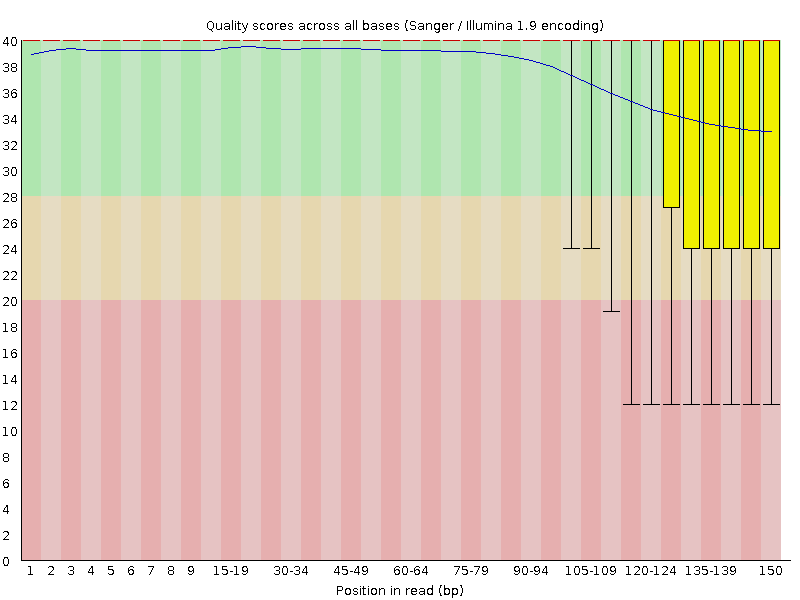
\includegraphics[width=\textwidth]{imagens/fastqc_R1_quality.png}
    \end{minipage}
    \hfill
    \begin{minipage}[t]{0.48\textwidth}
        \centering
        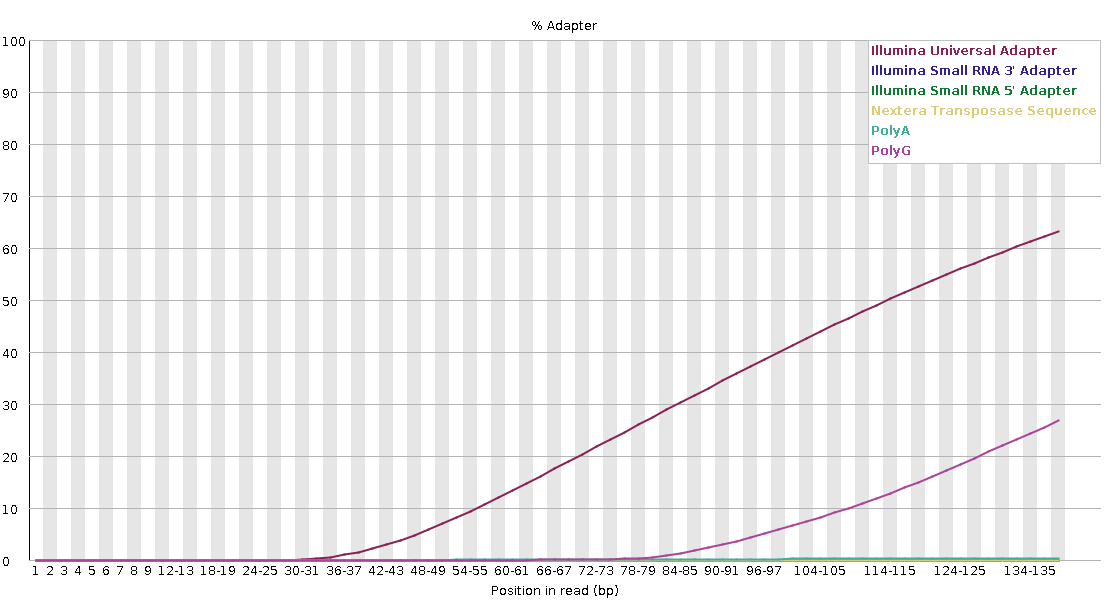
\includegraphics[width=\textwidth]{imagens/fastqc_R1_adapter.png}
    \end{minipage}

    \vspace{0.3cm}

    \begin{minipage}[t]{0.48\textwidth}
        \centering
        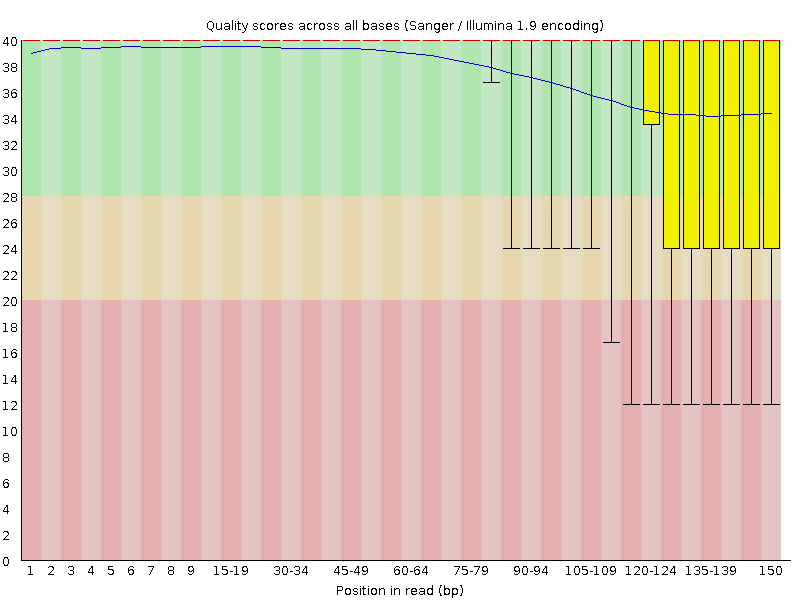
\includegraphics[width=\textwidth]{imagens/fastqc_R2_quality.png}
    \end{minipage}
    \hfill
    \begin{minipage}[t]{0.48\textwidth}
        \centering
        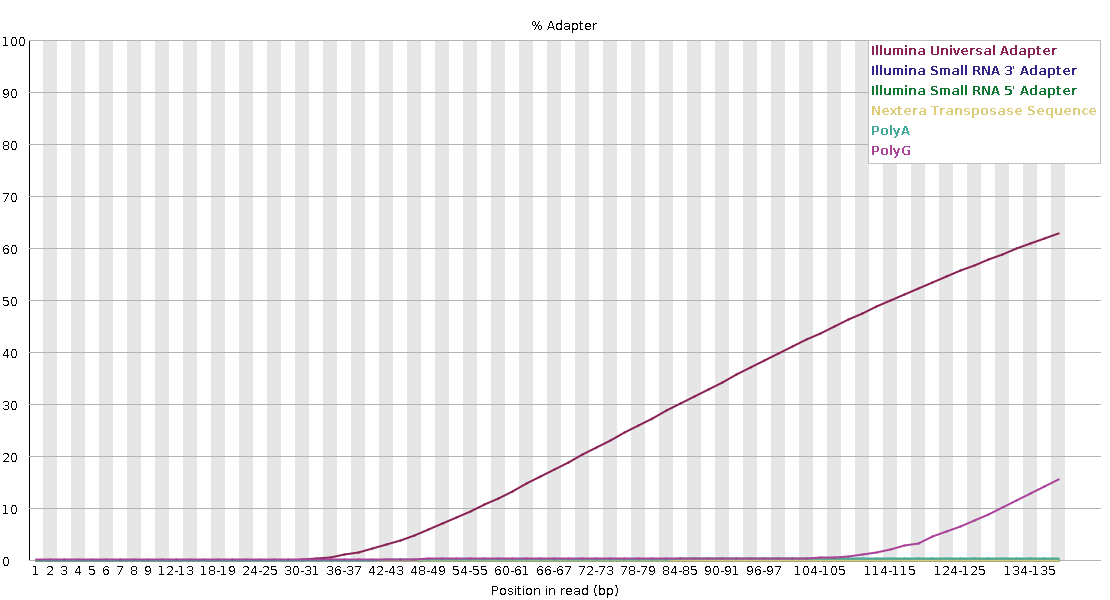
\includegraphics[width=\textwidth]{imagens/fastqc_R2_adapter.png}
    \end{minipage}
    \caption{Relatórios FastQC para a arara-azul-de-lear. Acima: R1 --- qualidade \textit{per-base} (esq.) e conteúdo de adaptadores (dir.). Abaixo: R2 --- qualidade \textit{per-base} (esq.) e conteúdo de adaptadores (dir.).}
    \label{fig:fastqc}
\end{figure}

\section{Montagem do Mitogenoma}

A montagem pelo NOVOPlasty resultou em genomas mitocondriais circularizados para ambas as espécies. A Tabela~\ref{tab:montagem} apresenta as métricas de montagem obtidas.

\begin{table}[H]
\centering
\caption{Métricas de montagem do mitogenoma para as duas espécies analisadas.}
\label{tab:montagem}
\footnotesize
\begin{tabular}{@{}lp{4.5cm}p{5cm}@{}}
\toprule
\textbf{Métrica} & \textbf{\textit{A.~leari}} & \textbf{\textit{D.~bifasciatus}} \\
\midrule
Tamanho & 16.986 bp & $\sim$16.800 bp (circularizado) \\
Circularização & Sim & Sim \\
K-mer ótimo & 39 & 33 \\
Cobertura média & 306$\times$ & não medida (dataset completo) \\
Reads alinhadas & 34.644 / 20.285.220 (0,17\%) & --- \\
Insert size medido & 213 bp (parametrizado: 300) & --- \\
Referência & 16.999 bp (\textit{A.~hyacinthinus}) --- $\Delta$ 13 bp & 16.805 bp (PZ143763.1) --- $\Delta$ $\sim$5 bp \\
\bottomrule
\end{tabular}
\end{table}

Para \textit{D.~bifasciatus}, o dataset compacto (12M reads, $\sim$1,2~GB) foi processado integralmente sem truncagem; a circularização ocorreu na primeira tentativa com k-mer 33. A etapa de anotação funcional (MITOS2) não foi executada para esta espécie no perfil de teste, que foi configurado sem o parâmetro \texttt{mitos2\_db} para demonstrar a modularidade do pipeline --- a Fase 1 (montagem) opera independentemente da Fase 2 (anotação). A validação da montagem pode ser realizada por BLAST contra a referência PZ143763.1.

O resultado da arara-azul-de-lear merece destaque: o genoma montado de 16.986 bp difere em apenas 13 pares de bases do mitogenoma de referência de \textit{A.~hyacinthinus} (16.999 bp, NC\_082165.1), demonstrando alta congruência interespecífica esperada para o gênero \textit{Anodorhynchus}. A cobertura média de 306$\times$ é amplamente superior ao mínimo recomendado de 30--50$\times$ para montagens confiáveis \cite{dierckxsens2017}, conferindo alta confiabilidade ao resultado.

A proporção de leituras mitocondriais de 0,17\% é condizente com a estimativa teórica para dados de genoma total de aves, onde o número de cópias mitocondriais por célula é tipicamente na ordem de centenas a milhares, mas o genoma nuclear ($\sim$1,2~Gb em psitacídeos) é muito maior que o mitocondrial ($\sim$17~kb).

O log do NOVOPlasty reportou uma fração de subamostragem (\textit{subsampled fraction}) de 61,9\%, indicando que o algoritmo processou 61,9\% das leituras de entrada antes de obter a circularização. Esse valor reflete a eficiência do \textit{seed-and-extend}: como o NOVOPlasty constrói o genoma iterativamente a partir da semente, ele pode alcançar a montagem completa sem necessidade de processar todas as leituras disponíveis, resultando em economia computacional proporcional à fração não processada.

\begin{figure}[H]
    \centering
    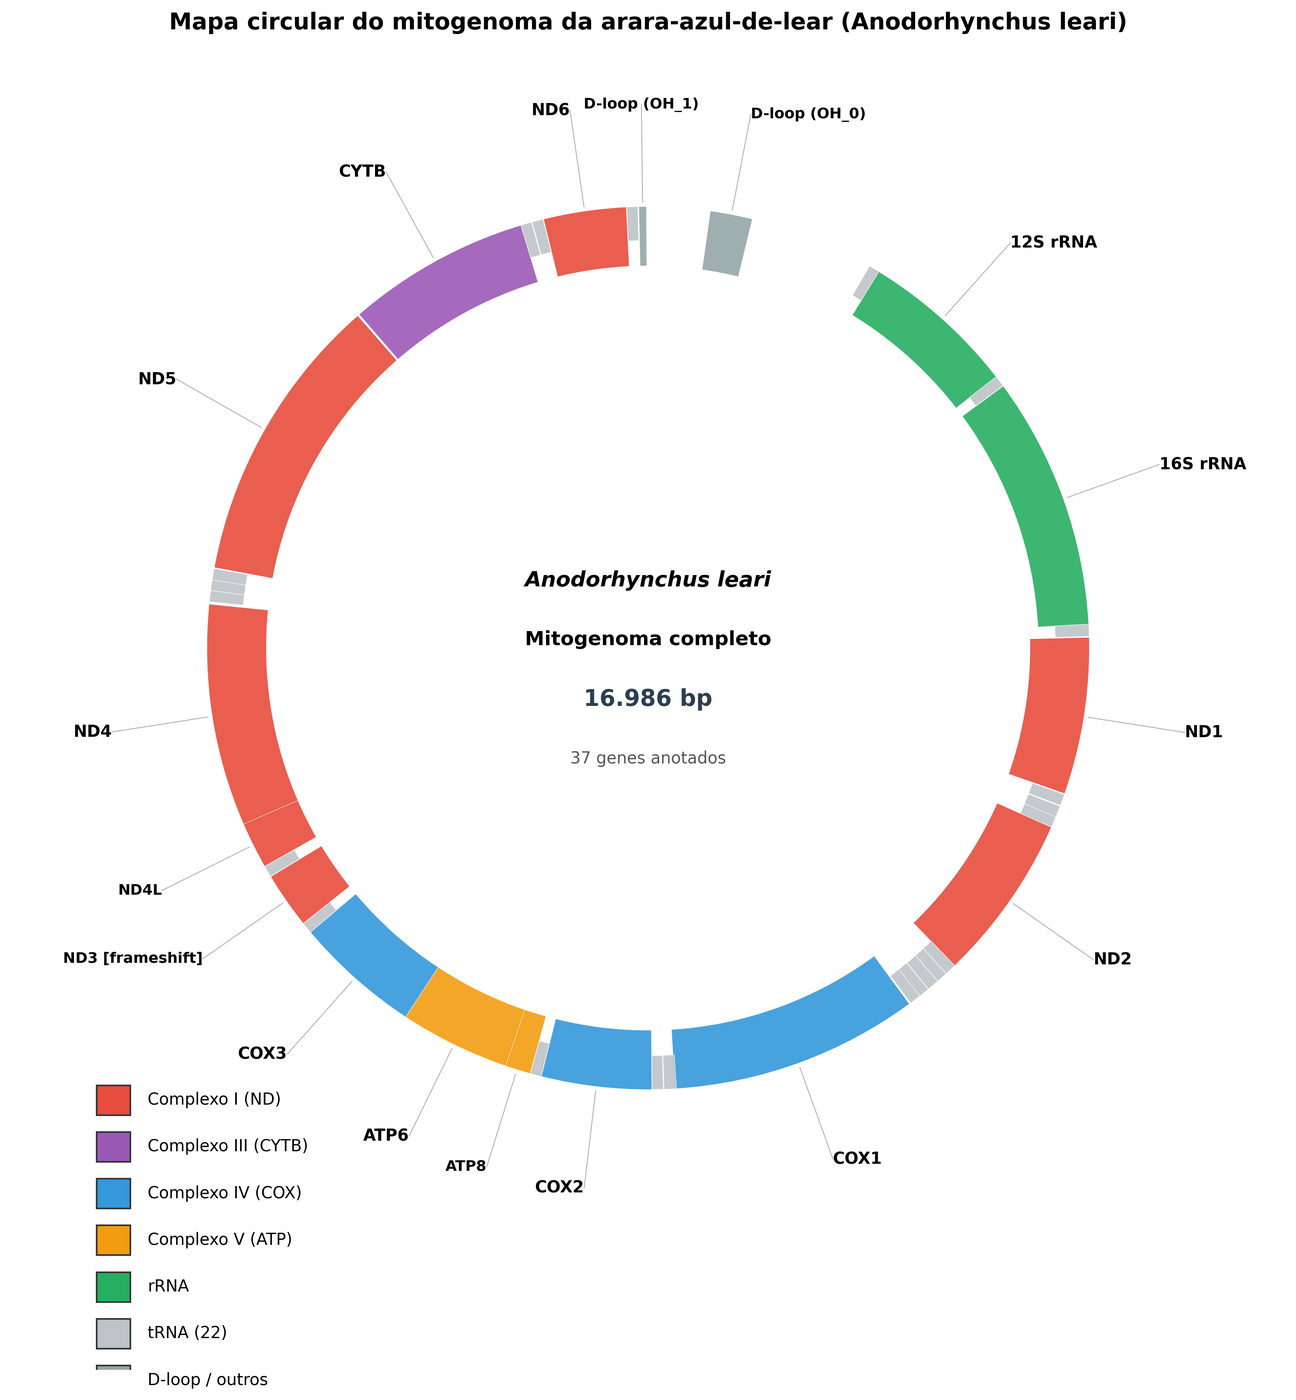
\includegraphics[width=0.70\textwidth]{imagens/mapa_circular_mitogenoma.png}
    \caption{Mapa circular do mitogenoma da arara-azul-de-lear (\textit{A.~leari}), mostrando a posição dos 37 genes (13 CDS, 22 tRNAs, 2 rRNAs) e a região controle (D-loop). Gerado automaticamente pelo pipeline via Biopython GenomeDiagram.}
    \label{fig:mapa_circular}
\end{figure}

\section{Anotação Funcional}

A anotação pelo MITOS2 identificou o conjunto completo de genes esperado para um genoma mitocondrial de ave, conforme apresentado na Tabela~\ref{tab:anotacao}.

\begin{table}[H]
\centering
\caption{Conteúdo gênico do mitogenoma da arara-azul-de-lear anotado pelo MITOS2.}
\label{tab:anotacao}
\begin{tabular}{@{}clp{9.5cm}@{}}
\toprule
\textbf{Tipo} & \textbf{Qtd.} & \textbf{Genes} \\
\midrule
CDS & 13 & nad1, nad2, nad3, nad4, nad4l, nad5, nad6, cox1, cox2, cox3, atp6, atp8, cob \\
\addlinespace
tRNA & 22 & tRNA-Phe, tRNA-Val, tRNA-Leu1, tRNA-Ile, tRNA-Gln, tRNA-Met, tRNA-Trp, tRNA-Ala, tRNA-Asn, tRNA-Cys, tRNA-Tyr, tRNA-Ser1, tRNA-Asp, tRNA-Lys, tRNA-Gly, tRNA-Arg, tRNA-His, tRNA-Ser2, tRNA-Leu2, tRNA-Glu, tRNA-Thr, tRNA-Pro \\
\addlinespace
rRNA & 2 & rrnS (12S), rrnL (16S) \\
\addlinespace
Origem de replicação & 2 & OH\_0, OH\_1 \\
\bottomrule
\end{tabular}
\end{table}

A ordem gênica identificada é compatível com o padrão conservado de Psittaciformes, corroborando a confiabilidade da montagem. A comparação com a anotação de \textit{A.~hyacinthinus} (NC\_082165.1) confirmou a conservação da organização gênica dentro do gênero. A completude e a consistência da anotação --- 13 CDS, 22 tRNAs com anticódons corretos, 2 rRNAs nas posições esperadas e nenhum gene truncado ou duplicado --- servem como validação biológica indireta da montagem: um genoma incorretamente circularizado ou contendo inserções e deleções artifactuais produziria genes com códons de parada prematuros, tRNAs com estruturas secundárias anômalas ou regiões intergênicas atipicamente longas --- nenhum dos quais foi observado.

\subsection{Caso Especial --- Frameshift do ND3}

Um aspecto biologicamente relevante revelado pela anotação é o tratamento do gene ND3. O MITOS2 reportou este gene como dois ORFs distintos (\texttt{nad3\_0} e \texttt{nad3\_1}) com sobreposição de 5~bp, refletindo o \textit{frameshift insertion} documentado por \citeonline{mindell1998} em genomas mitocondriais de aves. Esse fenômeno, em que uma inserção de $\sim$1 nucleotídeo altera o quadro de leitura no interior do gene, é corrigido \textit{in vivo} por mecanismos de \textit{programmed ribosomal frameshift} ou edição do mRNA. Na referência \textit{A.~hyacinthinus} (NC\_082165.1), o ND3 é anotado com \texttt{join()}:

\begin{lstlisting}
CDS   join(9504..9677,9679..9854)
      /gene="ND3"
      /note="frameshift mechanism unknown (Mindell et al., 1998)"
\end{lstlisting}

Para a conversão dos resultados ao formato GenBank Flat File, o script \texttt{gff2genbank\allowbreak.py} do pipeline detecta automaticamente a presença de \texttt{nad3\_0} e \texttt{nad3\_1} e os unifica em um único CDS com \texttt{join()}, aplicando o qualificador \texttt{/exception=\allowbreak ribosomal\allowbreak{} slippage} --- exatamente como exigido pelo GenBank para submissão. Quando a espécie não apresenta esse \textit{frameshift} (e.g., invertebrados), o ND3 é anotado normalmente como um CDS contínuo.

% Tabela de posição física dos genes será apresentada no Capítulo 6.

\begin{figure}[H]
    \centering
    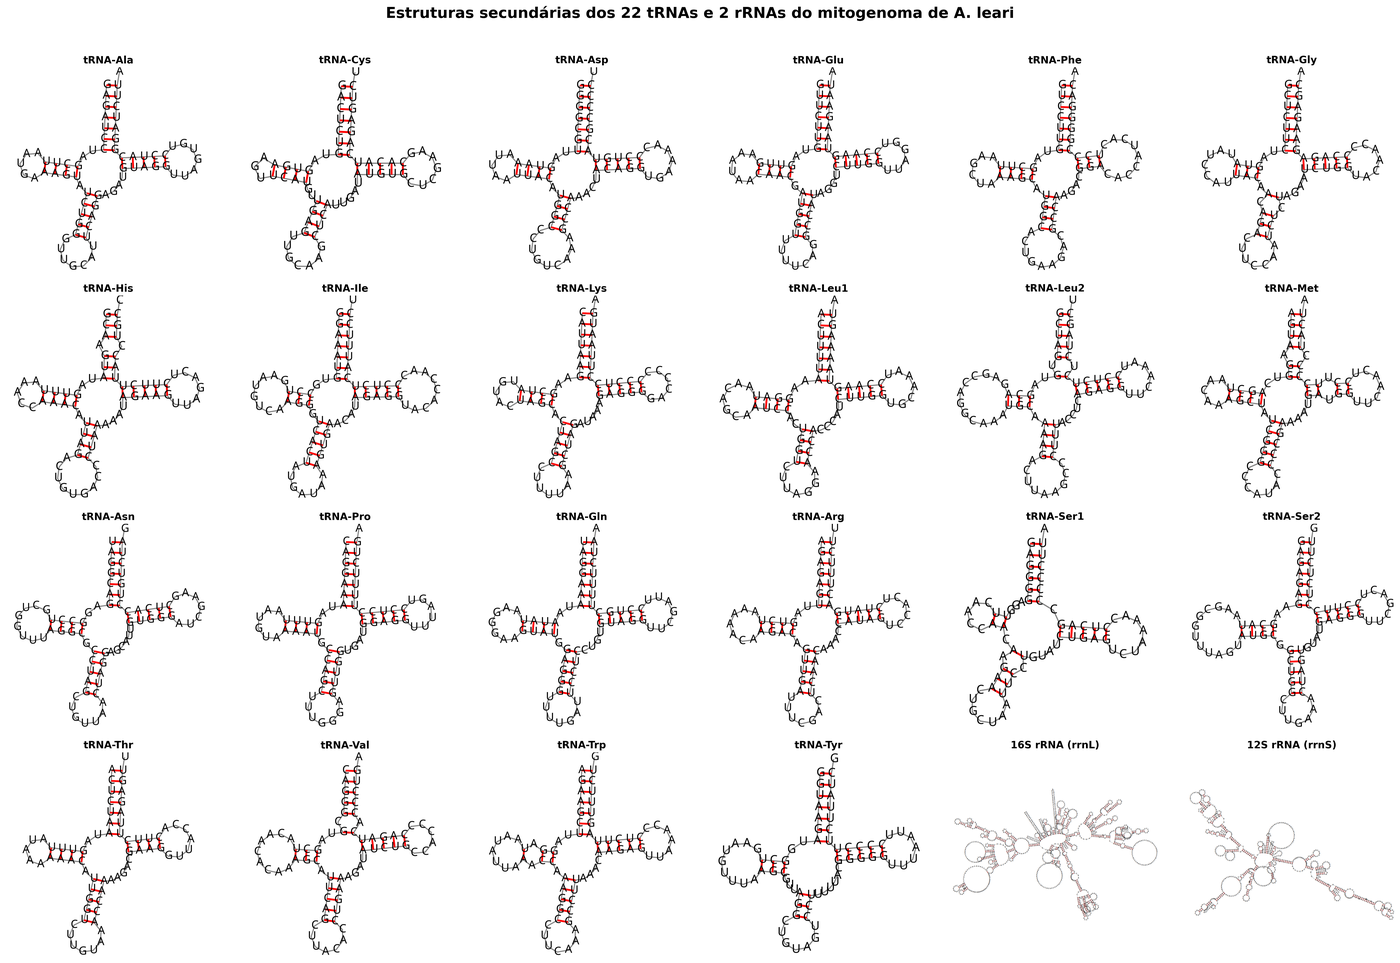
\includegraphics[width=\textwidth]{imagens/painel_trna_rrna.png}
    \caption{Painel com estruturas secundárias dos 22 tRNAs e 2 rRNAs preditos pelo MITOS2/RNAplot para \textit{A.~leari}. Nota-se a ausência do braço DHU no tRNA-Ser(AGY), padrão conservado em metazoários.}
    \label{fig:painel_trna_rrna}
\end{figure}

\section{Compilação dos Entregáveis e Formato GenBank}

O módulo COMPILE\_SUMMARY reuniu automaticamente todos os produtos da análise em uma pasta organizada com 14 categorias de entregáveis, conforme detalhado na Tabela da Seção~4.11. Destaca-se a geração automática do GenBank Flat File (\texttt{.gbk}), que é o formato padrão exigido pelo NCBI para submissão de genomas. O arquivo gerado para a arara-azul-de-lear contém:

\begin{lstlisting}[caption={Trecho do GenBank Flat File gerado pelo pipeline para \textit{A.~leari}.},label={lst:genbank}]
LOCUS       A_leari                16986 bp    DNA     circular VRT 12-APR-2026
DEFINITION  Anodorhynchus leari mitochondrion, complete genome.
ACCESSION   A_leari
VERSION     A_leari
FEATURES             Location/Qualifiers
     source          1..16986
                     /organism="Anodorhynchus leari"
                     /organelle="mitochondrion"
                     /mol_type="genomic DNA"
     ...
     CDS             join(10919..11098,11094..11267)
                     /gene="ND3"
                     /exception="ribosomal slippage"
                     /note="programmed frameshift; Mindell et al. (1998)"
     ...
ORIGIN
        1 gtttacgcta taaagcgtta gatataactg ...
//
\end{lstlisting}

Esse formato pode ser diretamente submetido ao GenBank via \texttt{table2asn} ou carregado em ferramentas de visualização como OGDRAW para geração de mapas circulares de alta qualidade.

\section{Análise de Desempenho e Eficiência Computacional}

A avaliação de desempenho de um pipeline bioinformático é essencial para determinar sua viabilidade prática em diferentes cenários de uso --- desde laptops pessoais até servidores de computação em nuvem. Em bioinformática, pipelines frequentemente processam volumes massivos de dados (dezenas a centenas de gigabytes), e compreender onde o tempo e os recursos computacionais são consumidos permite identificar gargalos, dimensionar infraestrutura adequada e estimar custos operacionais. Essa análise é particularmente relevante para laboratórios com recursos limitados, que precisam avaliar se dispõem de hardware suficiente antes de iniciar uma execução.

Nesta seção, são apresentadas métricas detalhadas de execução do pipeline para a arara-azul-de-lear, incluindo tempo, consumo de CPU, memória RAM e operações de entrada/saída (I/O) --- isto é, volume de dados lidos e escritos em disco --- por etapa. A partir dessas métricas, discutem-se a eficiência de cada módulo, a identificação de gargalos, o impacto do pré-processamento na qualidade da montagem, e o custo estimado de execução em infraestrutura de nuvem.

A execução foi realizada em um laptop com processador Intel Core i7-1165G7 (4 núcleos físicos, 8 threads via \textit{hyperthreading}, frequência base de 2,80~GHz), 16~GB de memória RAM DDR4 e armazenamento em estado sólido (SSD NVMe). O tempo total decorrido --- também chamado \textit{wall-clock time}, que mede o tempo real percebido pelo usuário, incluindo esperas por I/O e rede --- foi de \textbf{56 minutos e 42 segundos}, com consumo acumulado de \textbf{4,2 horas de CPU} (tempo efetivo de processamento somado de todos os núcleos). A Tabela~\ref{tab:desempenho} apresenta as métricas detalhadas por etapa.

\begin{table}[H]
\centering
\caption{Métricas de desempenho por etapa do pipeline (execução arara-azul-de-lear, 50M reads).}
\label{tab:desempenho}
\resizebox{\textwidth}{!}{%
\begin{tabular}{@{}lrrrrrr@{}}
\toprule
\textbf{Etapa} & \textbf{Tempo (min)} & \textbf{\% total} & \textbf{CPU (\%)} & \textbf{RAM pico (GB)} & \textbf{I/O leitura} & \textbf{I/O escrita} \\
\midrule
SRA\_PILOT & 1,9 & 3,4\% & 113\% & 0,15 & 3,4 MB & 474 MB \\
SRA\_DOWNLOAD & 33,8 & 59,6\% & 586\% & 0,43 & 160 GB & 250 GB \\
FASTQC & 7,6 & 13,4\% & 1966\% & 1,04 & 34,7 GB & 4,8 MB \\
TRIM\_GALORE & 12,2 & 21,5\% & 2084\% & 0,12 & 68,5 GB & 53,4 GB \\
NOVOPLASTY & 4,5 & 8,0\% & 827\% & 11,11 & 18 GB & 28 KB \\
MITOS2 & 4,1 & 7,2\% & 1033\% & 0,41 & 222 MB & 45 MB \\
\midrule
\textbf{Total} & \textbf{56,7} & \textbf{100\%} & --- & --- & --- & --- \\
\bottomrule
\end{tabular}}%
\end{table}

\begin{figure}[H]
    \centering
    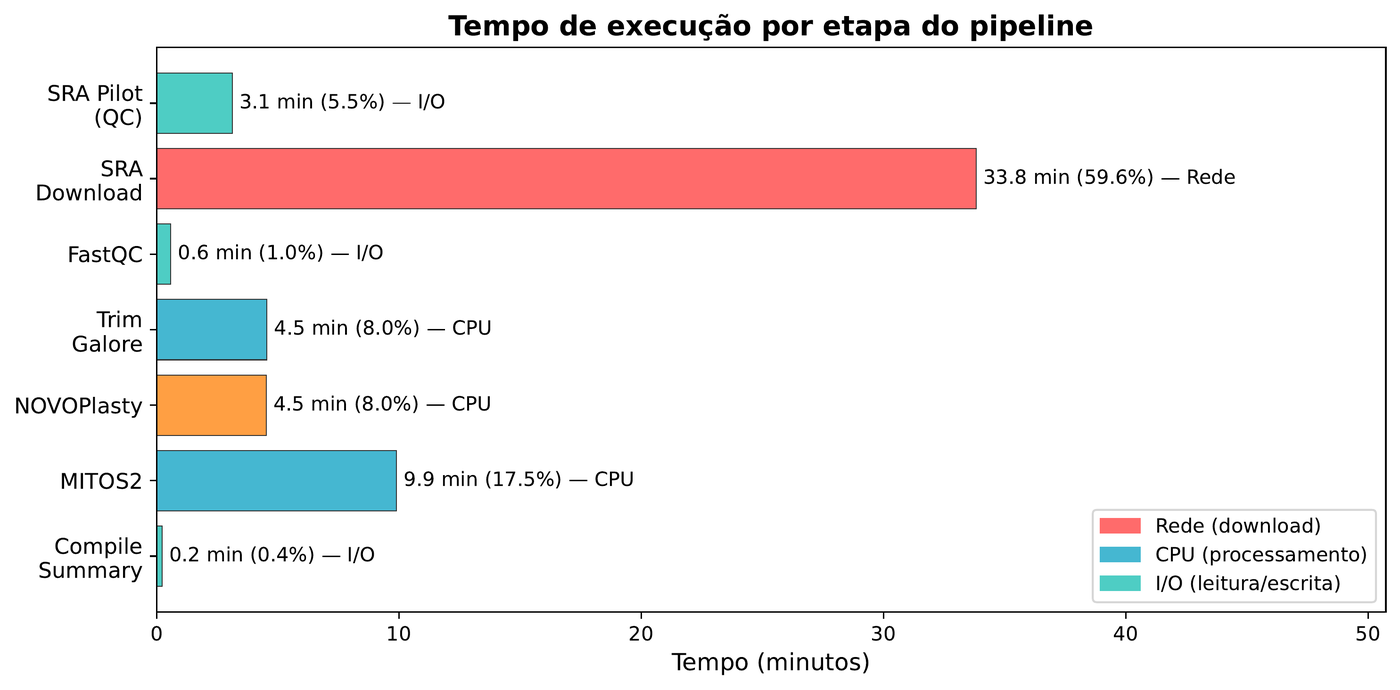
\includegraphics[width=0.85\textwidth]{imagens/tempo_etapas_pipeline.png}
    \caption{Tempo de execução por etapa do pipeline para a arara-azul-de-lear, com anotação da porcentagem do tempo total e classificação por tipo de operação (I/O-bound vs CPU-bound).}
    \label{fig:tempo_etapas}
\end{figure}

\subsection{Gargalo de I/O: Download e Conversão SRA}

O download do SRA é o gargalo dominante, consumindo \textbf{59,6\% do tempo total}. A etapa engloba três operações sequenciais: \texttt{prefetch} (download do arquivo \texttt{.sra} comprimido, $\sim$11~GB), \texttt{fasterq-dump} (conversão para FASTQ, gerando $\sim$87~GB intermediários para 118M reads), e truncamento via \texttt{head} (redução para 50M reads). O volume total de I/O desta etapa (160~GB lidos + 250~GB escritos) confirma que a conversão de formato é o fator limitante, não a rede --- o \texttt{fasterq-dump} precisa descomprimir e reescrever todos os 118M reads mesmo que apenas 50M sejam necessários, pois o formato \texttt{.sra} não permite acesso aleatório por read.

Esse comportamento reforça a importância do módulo Pilot QC, que utiliza \texttt{fastq-dump\allowbreak{} -X\allowbreak{} 500000} para amostrar apenas as primeiras 500K reads diretamente da origem (sem download completo), consumindo apenas 1,9 minutos e 474~MB. Sem o Pilot, o usuário precisaria decidir arbitrariamente quantas reads baixar, arriscando sub ou superamostragem.

\subsection{Eficiência do Pré-processamento}

O Trim Galore consumiu 12,2 minutos (21,5\% do tempo), processando 100 milhões de reads (50M pares). A taxa de remoção de adaptadores foi de 81,4\% (R1) e 80,8\% (R2), com remoção de bases por qualidade inferior a 1\% (74M bp em R1, 51M bp em R2). Do total de 50M pares, 3.711.983 (7,42\%) foram removidos por ficarem abaixo de 50~bp após trimming --- indicando dímeros de adaptador. O volume de dados foi reduzido de 15~Gbp brutos para 10,78~Gbp filtrados (71,9\% de retenção em bases).

Uma questão pertinente é: \textbf{o trimming é necessário ou é perda de tempo?} A resposta é inequívoca: com 81,4\% dos reads contendo adaptador Illumina TruSeq, executar a montagem sem trimming resultaria em k-mers quiméricos (parte sequência biológica, parte adaptador sintético) que impediriam a extensão correta do grafo de Bruijn. Os 12,2 minutos de trimming ($\sim$21\% do pipeline) previnem artefatos de montagem que poderiam resultar em falha de circularização ou contigs espúrios. Em contraste, a montagem pós-trimming completou em apenas 4,5 minutos, com circularização na primeira tentativa.

O FASTQC rodou em paralelo com o Trim Galore (ambos consomem os mesmos FASTQs), não adicionando tempo ao caminho crítico. O pico de memória do FASTQC (1,04~GB) é significativo para máquinas com pouca RAM, mas justificável pela geração de relatórios de qualidade essenciais para verificação posterior.

\subsection{Anomalia de Memória do NOVOPlasty}

O NOVOPlasty apresentou o maior consumo de memória entre todas as etapas: \textbf{11,1~GB de RAM} (pico). Embora inferior aos 16~GB de memória física do sistema, esse valor --- somado ao consumo do sistema operacional, Docker e demais processos residentes ($\sim$3--4~GB) --- aproximou-se do limite total, resultando em uso pontual de \textit{swap}. O alto consumo decorre da construção do \textit{hash} de k-mers em memória para as 46M reads remanescentes. O NOVOPlasty, escrito em Perl, não possui gerenciamento granular de memória, e o parâmetro \texttt{Max memory} (configurado como 12~GB) serve apenas como limite superior sugerido, não como restrição efetiva.

A fração ``subsampled'' de 22,93\% reportada no log indica que o NOVOPlasty sub-amostrou internamente os dados de entrada, processando efetivamente $\sim$10,6M reads dos 46,3M disponíveis. Mesmo com essa sub-amostragem, a cobertura final de 306$\times$ é 6$\times$ superior ao mínimo recomendado de 50$\times$ \cite{dierckxsens2017}. Esse é um indicador relevante: com metade das reads (25M em vez de 50M), a montagem provavelmente ainda seria bem-sucedida, com cobertura estimada de $\sim$150$\times$.

\textbf{Recomendação prática:} para execução em máquinas com menos de 8~GB de RAM, reduzir o \texttt{sra\_max\_reads} para 20M ou configurar \texttt{Max memory = 6} no perfil Nextflow. A qualidade da montagem não seria comprometida.

\subsection{Cascata de Redução de Dados}

Uma análise particularmente reveladora é a redução progressiva do volume de dados ao longo do pipeline. A Tabela~\ref{tab:cascata} apresenta essa cascata de redução.

\begin{table}[H]
\centering
\caption{Cascata de redução de dados ao longo do pipeline.}
\label{tab:cascata}
\begin{tabular}{@{}lrrr@{}}
\toprule
\textbf{Etapa} & \textbf{Volume} & \textbf{Fator de redução} & \textbf{Acumulado} \\
\midrule
SRA completo (118,5M reads) & $\sim$87 GB & --- & 1$\times$ \\
Após truncamento (50M reads) & $\sim$42 GB & 2,1$\times$ & 2,1$\times$ \\
Após trimming (46,3M reads) & $\sim$10,8 GB & 3,9$\times$ & 8,1$\times$ \\
Montagem circularizada & 17 KB & 635.000$\times$ & $\sim$5.100.000$\times$ \\
Summary (todos entregáveis) & 1,6 MB & --- & $\sim$54.000$\times$ \\
\bottomrule
\end{tabular}
\end{table}

O dado original (87~GB de FASTQ bruto) é reduzido em mais de \textbf{cinco milhões de vezes} até a montagem final (17~KB). Essa cascata demonstra que a maior parte do sequenciamento WGS é irrelevante para o genoma mitocondrial --- apenas 0,17\% das reads alinham ao mitogenoma. A existência do Pilot QC como primeira etapa evita o download desnecessário: em vez de baixar os 87~GB completos, o pipeline determina automaticamente que 50M reads ($\sim$42~GB) são suficientes.

\begin{figure}[H]
    \centering
    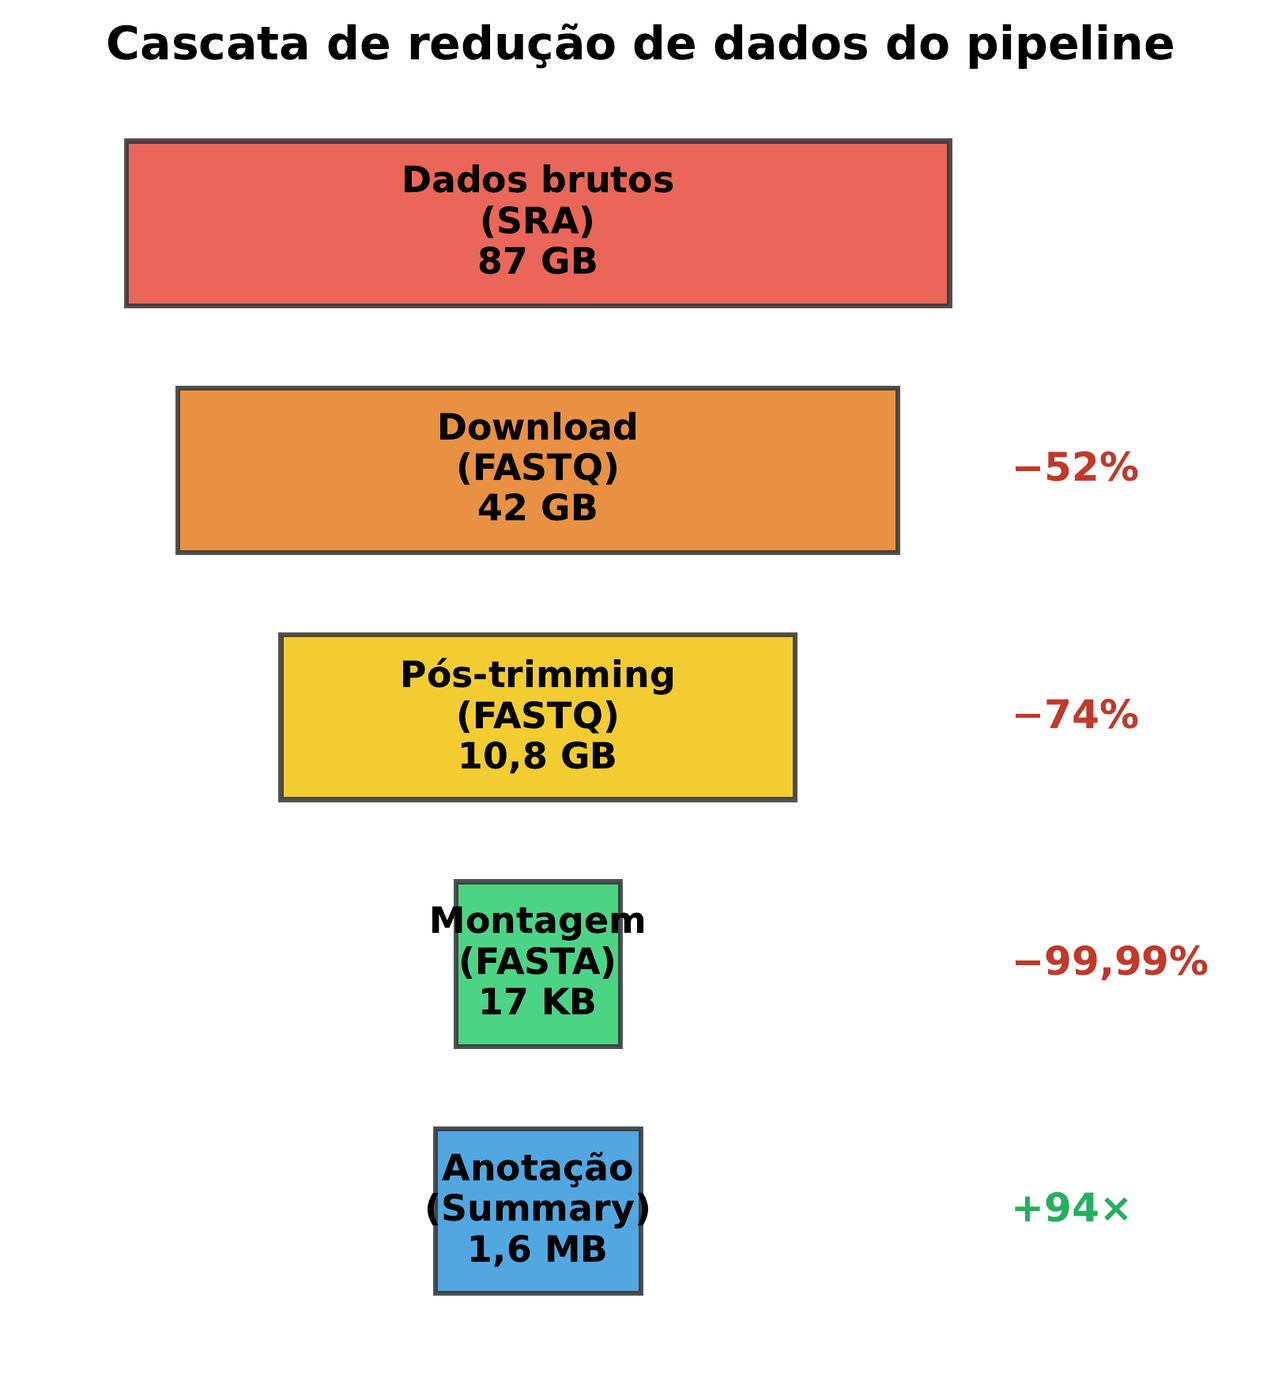
\includegraphics[width=0.85\textwidth]{imagens/funil_reducao_dados.png}
    \caption{Cascata de redução de dados ao longo do pipeline: de 87~GB de FASTQ bruto até 17~KB de genoma circularizado --- uma redução de aproximadamente 5 milhões de vezes.}
    \label{fig:funil_reducao}
\end{figure}

\subsection{Pico de Armazenamento e Custo Computacional}

Um aspecto frequentemente negligenciado em pipelines bioinformáticos é o \textbf{consumo de armazenamento durante a execução}, que pode ser significativamente maior que o tamanho dos resultados finais. Isso ocorre porque as etapas intermediárias geram arquivos temporários volumosos (FASTQs descomprimidos, arquivos de cache) que são consumidos pelas etapas seguintes e depois descartados.

No caso da execução para a arara-azul-de-lear, o pico de uso de disco foi de \textbf{27~GB} no diretório de trabalho, dominado pela etapa SRA\_DOWNLOAD (23~GB de FASTQs descomprimidos e cache \texttt{.sra}). Em contraste, ao final da execução, os resultados úteis ocupam apenas \textbf{$\sim$67~MB} em \texttt{results/}. Os arquivos intermediários podem ser removidos com o comando \texttt{nextflow clean}, liberando o espaço ocupado. Essa diferença de $\sim$400$\times$ entre o pico de armazenamento e os resultados finais é uma característica importante a considerar ao dimensionar a infraestrutura.

\textbf{Custo computacional em hardware doméstico.} Todo o pipeline foi executado em um notebook pessoal com processador de 4 núcleos, 16~GB de RAM e disco SSD convencional. Os requisitos computacionais reais observados foram:

\begin{itemize}
    \item \textbf{Processamento:} 56,7 minutos de tempo total (\textit{wall-clock}), com pico de uso de 4 threads durante a conversão SRA e o trimming. Nenhuma etapa exigiu processamento de alto desempenho --- o processo mais intensivo (NOVOPlasty) utilizou apenas 1 thread.
    \item \textbf{Armazenamento:} 27~GB de pico no diretório de trabalho, reduzidos a $\sim$67~MB de resultados finais após limpeza dos arquivos temporários. Um disco com pelo menos 50~GB livres é suficiente com margem de segurança.
    \item \textbf{Memória RAM:} pico de 11,1~GB durante a montagem com NOVOPlasty, dentro dos 16~GB disponíveis. Um computador com 8~GB de RAM pode apresentar lentidão nessa etapa, mas não é impedido de executá-la.
    \item \textbf{Rede:} o download do arquivo SRA ($\sim$11~GB) foi o principal consumidor de banda, com duração variável conforme a velocidade da conexão.
\end{itemize}

Esses requisitos modestos demonstram que \textbf{a montagem e anotação de mitogenomas não exige infraestrutura computacional especializada}. Qualquer computador pessoal de categoria intermediária, com 16~GB de RAM, disco SSD e acesso à internet, é capaz de executar o pipeline completo em menos de uma hora. Essa acessibilidade é particularmente relevante para estudantes e grupos de pesquisa com recursos limitados, que podem reproduzir integralmente os resultados deste trabalho sem investimento adicional em hardware.

\subsection{Caminho Crítico e Otimização Implementada}

O \textbf{caminho crítico} de um pipeline --- ou seja, a sequência de etapas dependentes que determina o tempo mínimo de execução --- é: SRA\_PILOT $\rightarrow$ SRA\_DOWNLOAD $\rightarrow$ TRIM\_GALORE $\rightarrow$ NOVOPLASTY $\rightarrow$ MITOS2 $\rightarrow$ COMPILE\_SUMMARY. Etapas que executam em paralelo, como o FASTQC (que processa os mesmos FASTQs que o Trim Galore ao mesmo tempo), \textbf{não adicionam tempo ao caminho crítico}, exceto quando excedem a duração da etapa paralela. No caso observado, o FASTQC (7,6~min) completou antes do Trim Galore (12,2~min) e, portanto, não impactou o tempo total.

A análise do caminho crítico revela que \textbf{81,1\% do tempo total} (46 de 56,7~min) é consumido por apenas duas etapas: download/conversão SRA (33,8~min) e trimming (12,2~min). A montagem em si --- o objetivo central do pipeline --- leva apenas 4,5 minutos (8,0\%), demonstrando que o gargalo real não é computacional, mas de transferência e transformação de dados.

A partir dessa análise, foi identificada e implementada uma otimização concreta. A análise da sub-amostragem interna do NOVOPlasty (Seção~5.7.3) revelou que apenas 22,93\% das reads foram efetivamente utilizadas na montagem. Isso indica que o limite anteriormente definido (50 milhões de reads) era excessivamente conservador: com 25 milhões de reads, a cobertura estimada seria de $\sim$150$\times$ --- ainda 3$\times$ acima do mínimo recomendado na literatura \cite{dierckxsens2017}. Com base nessa evidência, o limite máximo do módulo Pilot QC foi reduzido de 50 milhões para 25 milhões de reads, diminuindo proporcionalmente o tempo de download, conversão e trimming. A estimativa de tempo total com essa otimização é de $\sim$35 minutos --- uma redução de 38\% em relação à execução observada --- sem comprometer a qualidade da montagem.

\subsection{Síntese da Análise de Desempenho}

A análise de desempenho revelou três conclusões principais sobre o comportamento computacional do pipeline:

\textbf{O gargalo é I/O, não processamento.} Das sete etapas do pipeline, a montagem do mitogenoma --- objetivo central do trabalho --- consome apenas 8\% do tempo total (4,5~min). O restante é dominado por operações de transferência e transformação de dados: o download e conversão do SRA representam 59,6\% (33,8~min) e o trimming responde por 21,5\% (12,2~min). Em termos práticos, isso significa que melhorias na velocidade de rede ou na estratégia de amostragem têm impacto muito maior no tempo total do que otimizações no algoritmo de montagem.

\textbf{A etapa de trimming justifica seu custo.} Apesar de consumir 12 minutos, o trimming não é dispensável: 81,4\% das reads continham sequências de adaptadores que, se mantidas, poderiam gerar extensões quiméricas no grafo do NOVOPlasty. Os 12 minutos investidos previnem falhas de circularização que exigiriam re-execução completa do pipeline --- um custo muito superior.

\textbf{Sem as estratégias implementadas no pipeline, a montagem de um mitogenoma a partir de dados públicos seria inviável em hardware doméstico.} O dataset original de \textit{A.~leari} (SRR28399504) contém 118,5 milhões de pares de leituras, que, quando convertidos para o formato FASTQ, ocupam aproximadamente 87~GB de espaço em disco. Carregar e processar esse volume na íntegra --- como seria necessário em uma abordagem manual sem truncamento --- exigiria centenas de gigabytes de armazenamento temporário (leitura, escrita intermediária e saída), além de memória RAM proporcional ao volume de dados nos estágios de trimming e montagem. Um notebook convencional com 16~GB de RAM e 256~GB de SSD simplesmente não comportaria essa carga; seria necessário recorrer a um servidor dedicado ou a uma infraestrutura de computação em nuvem.

O pipeline resolve esse problema por meio de uma cadeia de reduções progressivas que viabilizam a execução em hardware modesto. O \textbf{Pilot QC} analisa uma amostra mínima (500 mil leituras, $\sim$500~MB) e calcula exatamente quantas leituras são necessárias para atingir a cobertura-alvo, evitando o download do dataset inteiro. O \textbf{truncamento} reduz o volume de 87~GB para $\sim$21~GB (apenas 25 milhões de pares). O \textbf{trimming} remove adaptadores e bases de baixa qualidade, reduzindo para $\sim$10,8~GB de dados úteis. Finalmente, o \textbf{NOVOPlasty} sub-amostra internamente e opera apenas sobre as leituras que alinham à semente, consumindo uma fração do total. O resultado: de 87~GB de dados brutos, o pipeline extrai um mitogenoma de \textbf{17~KB} --- uma redução de aproximadamente 5 milhões de vezes.

Essa cadeia de decisões é o que torna possível executar o ciclo completo --- do dado bruto público ao mitogenoma anotado com 14 categorias de entregáveis --- em aproximadamente 35 minutos, em um notebook com 4 núcleos e 16~GB de RAM, sem necessidade de infraestrutura especializada. A viabilidade em hardware doméstico é particularmente relevante para estudantes de graduação e pesquisadores em instituições com recursos computacionais limitados, que de outra forma dependeriam de acesso a servidores ou clusters para realizar análises genômicas.

% A Figura~\ref{fig:tempo_etapas} já apresenta o detalhamento do tempo por etapa.

\section{Discussão sobre a Robustez da Abordagem}

A execução bem-sucedida do pipeline para duas espécies distintas --- uma ave (Psittaciformes) e um peixe (Perciformes) ---, utilizando datasets de plataformas diferentes (HiSeq X Ten e NovaSeq X Plus), demonstra a generalização da abordagem. A obtenção de genomas circularizados em ambos os casos, com o conjunto completo de 37 genes identificados no caso anotado, valida tanto o fluxo de montagem quanto a integração de ferramentas.

A cobertura de 306$\times$ obtida para \textit{A.~leari} com apenas 0,17\% de leituras mitocondriais em 20 milhões de pares demonstra que o DNA mitocondrial é eficientemente recuperado pelo NOVOPlasty mesmo quando representa uma fração diminuta do total de dados, confirmando as observações da literatura \cite{dierckxsens2017}.

A combinação metodológica adotada neste trabalho --- NOVOPlasty para montagem e MITOS2 para anotação --- corresponde ao padrão predominante na literatura recente de genômica mitocondrial, empregada em estudos abrangendo desde 213 mitogenomas de lagartos \cite{zhan2024} até espécies individuais de peixes \cite{kundu2024}, arraias \cite{guerreiro2025} e invertebrados \cite{shi2024,tao2024}. Essa convergência metodológica independente --- em que grupos de pesquisa de diferentes países, trabalhando com táxons distintos, adotam as mesmas ferramentas --- constitui uma validação externa da abordagem e reforça a confiabilidade das escolhas implementadas no pipeline.

A lógica iterativa de montagem com re-seeding automático e múltiplos k-mers mostrou-se eficaz, circularizando na primeira tentativa (k-mer 39) para \textit{A.~leari} e na primeira tentativa (k-mer 33) para \textit{D.~bifasciatus}. Essa robustez é particularmente relevante para cenários em que a \textit{seed} disponível é de uma espécie distante, ou quando regiões repetitivas dificultam a circularização.

O módulo Pilot QC foi validado por meio de execução isolada do script \texttt{pilot\_qc.sh} sobre uma subamostra de 100.000 leituras de \textit{A.~leari}, extraída do dataset SRR28399504. A análise piloto detectou qualidade Q30 de 86,2\%, taxa de adaptador de 66,4\% e fração mitocondrial estimada de 0,17\% (via correspondência de k-mers com a semente cox1). Com esses valores, a recomendação automática foi de 36 milhões de leituras para atingir 500$\times$ de cobertura --- resultado coerente com os 306$\times$ efetivamente obtidos com 20 milhões de leituras na execução principal. A configuração de produção do perfil \texttt{a\_leari} não define \texttt{sra\_max\_reads}, ativando o Pilot QC automaticamente em execuções futuras. Essa funcionalidade é particularmente valiosa para pesquisadores trabalhando com espécies pouco caracterizadas, onde não há estimativa prévia da fração mitocondrial.

Em comparação com os trabalhos relacionados, o pipeline desenvolvido apresenta vantagens claras em termos de reprodutibilidade, portabilidade e acessibilidade computacional. Enquanto o MitoHiFi \cite{ulianosilva2023} utiliza Conda para gerenciamento de dependências, sujeito a variações de ambiente, e o MITObim \cite{hahn2013} e o GetOrganelle \cite{jin2020} dependem de configuração manual, o pipeline aqui proposto encapsula todas as ferramentas em containers Docker com versões pinadas e orquestra sua execução via Nextflow, garantindo resultados idênticos em qualquer ambiente. Adicionalmente, as soluções existentes não incorporam mecanismos de redução automática do volume de dados, pressupondo que o usuário disponha de infraestrutura com armazenamento e memória suficientes para processar datasets completos --- requisito que exclui a maioria dos computadores pessoais. O pipeline aqui proposto, ao integrar o Pilot QC e o truncamento adaptativo, elimina essa barreira e permite que o ciclo completo --- do dado bruto ao mitogenoma anotado --- seja executado em um notebook convencional. A adição da Fase 2 (anotação funcional com MITOS2 e geração automática de entregáveis em formato GenBank) vai além do que a maioria dos pipelines de montagem de organelas oferece, cobrindo o ciclo completo desde o dado bruto até a submissão ao banco de dados.

Os resultados metodológicos apresentados neste capítulo demonstram que o pipeline é funcional, eficiente e acessível. O capítulo seguinte dedica-se integralmente à espécie-alvo deste trabalho --- a arara-azul-de-lear ---, explorando em profundidade o mitogenoma obtido, sua organização gênica e as implicações para a conservação da espécie.
